\begin{figure}[t]
\centering
\begin{tabular}{@{}c c c c@{}}
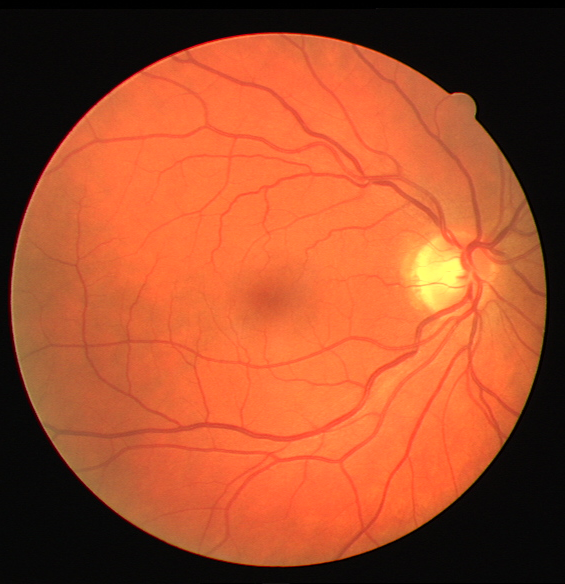
\includegraphics[width=0.24\columnwidth]{\figpath/retina/02_test} &
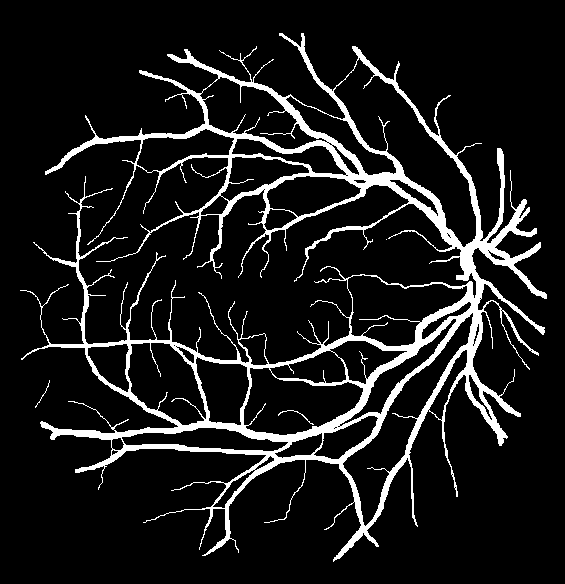
\includegraphics[width=0.24\columnwidth]{\figpath/retina/02_manual1_pos} &
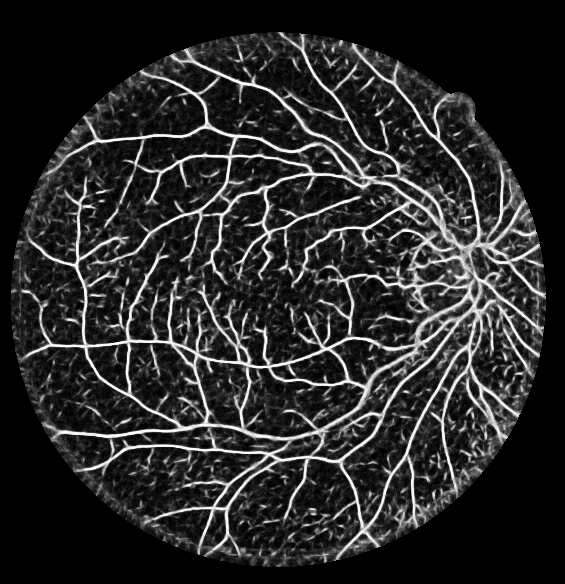
\includegraphics[width=0.24\columnwidth]{\figpath/retina/02_segmentation} &
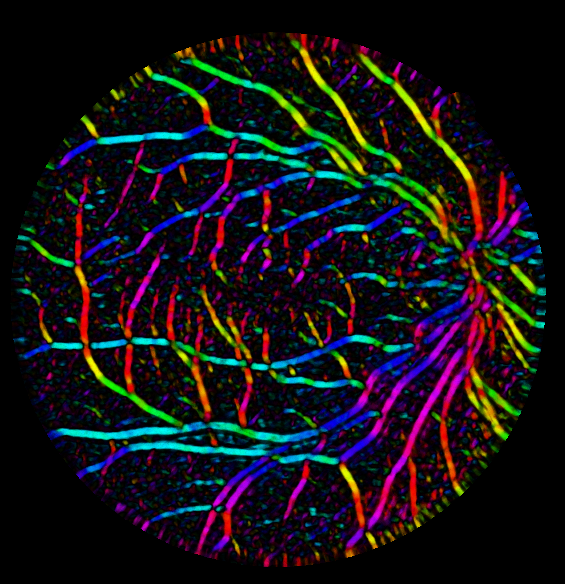
\includegraphics[width=0.24\columnwidth]{\figpath/retina/002_orientation_mag} \\
(a) & (b) & (c) & (d)\\
\noalign{\smallskip}
\end{tabular}
%
\caption{Estimating orientation in retinography: %
(a) input image; %
(b) ground truth mask indicating pixels belonging to a vessel; %
(c,d) vessel segmentation and orientation estimation using random forests and \dtcwt{} features. In (d), hue and brightness indicate the angle and magnitude of the predicted orientation vector. %
}
\label{f:retinography}
\end{figure}
